%================================================================================
% Erstellt am: 		10.07.2008
% Überarbeitet am:	08.07.2009
% Autor:			Holger Fischer
%
% Kann frei für Bachelor-/Diplom-/Masterarbeiten verwendet werden.
% Viel Erfolg!!!
%=====================================\textbf{}===========================================

%Einbinden der Datei header.tex; diese enthält alle verwendeten Pakete,
%sowie Änderungen am Layout
%!TEX root = ../Dokumentation.tex

%Da Latex für englischsprachige Texte ausgerichtet ist,
%wird als Dokumentenklasse das "`scrbook"' von Markus Kohm verwendet.
%Dieses ist für deutschsprachige Texte ausgelegt.
%BCOR12mm: 12mm Bindekorrektur (Verbreiterung des linken Randes)
%DIV11: entspricht in etwas der geforderten Textgröße und Seitenränder
%titlepage: eine Titelseite wird verwendet
%a4paper: DIN A4
%oneside: für eine spätere einseitige Bedruckung 
%Original: \documentclass[BCOR12mm,DIV11,titlepage,a4paper,oneside]{scrbook}
\documentclass[DIV11,titlepage,a4paper,oneside]{scrbook}

\textheight = 23cm

%Paket für deutsche Silbentrennung etc.
\usepackage{ngerman}

%Paket für Zeichenkodierung, entspricht UTF-8
\usepackage[utf8x]{inputenc}

%Paket das die Ausgabefonts definiert
\usepackage[T1]{fontenc}

%Paket für das Einbinden von Grafiken über die figure-Umgebung
\usepackage{graphicx}

%Paket verhindert floating
\usepackage[section]{placeins}

%Paket zum Ändern der Listenabstände
\usepackage{enumitem}
\setlist[itemize]{itemsep=0mm}
\setlist[enumerate]{itemsep=0mm}

%Paket zum Ändern der Kopf- und Fußzeile
\usepackage{fancyhdr}

%fancypagestyle{fancy}
\renewcommand{\headrulewidth}{0pt}
\fancyhf{}
%\fancyfoot[L]{FANCY}
\fancyfoot[R]{\thepage}

\fancypagestyle{plain}{
	\renewcommand{\headrulewidth}{0pt}
	\fancyhf{}
%	\fancyfoot[L]{PLAIN}
	\fancyfoot[R]{\thepage}
}

\pagestyle{plain}

%Abbildungsnummerierung ändern (abhängig von chapter, z.B. Abbildung 1.1)
\renewcommand*{\thefigure}{\thechapter.\arabic{figure}}
%Tabellennummerierung ändern (abhängig von chapter, z.B. Tabelle 1.1)
\renewcommand*{\thetable}{\thechapter.\arabic{table}}

%Paket, um ein Glossar/Abkürzungsverzeichnis anzulegen
\usepackage{nomencl}
\let\abbrev\nomenclature
%Der Name wird in Glossar geändert
\renewcommand{\nomname}{Glossar (optional)}
%Definiert die Aufteilung im Glossar zwischen Begriffen und Erläuterung
\setlength{\nomlabelwidth}{.25\hsize}
%Definiert die Punktelinien im Glossar
\renewcommand{\nomlabel}[1]{#1 \dotfill}
\setlength{\nomitemsep}{-\parsep}
%Veranlasst die Erstellung des Glossars
\makenomenclature

%Einrückungen nach Absätzen und Grafiken verhindern
\setlength{\parindent}{0pt}

%Verhindern, dass eine neue Seite für ein einzelnes Wort/Zeile verwendet wird
\clubpenalty = 10000 % schliesst Schusterjungen aus 
\widowpenalty = 10000 % schliesst Hurenkinder aus (keine Beleidigung, sondern wirklich ein Fachbegriff)

%Paket für ein deutsches Literaturverzeichnis
\usepackage{bibgerm}

%Paket für die Verwendung von URLs durch den Befehl \url{}
\usepackage{url}

%Paket für Zeilenabstand (onehalfspace, singlespace)
\usepackage{setspace}

%Paket zur Erzeugung von Anführungszeichen durch \enquote{Text}
\usepackage[ngerman]{babel}
\usepackage[babel, german=quotes]{csquotes}

%Paket für farbigen Text
%black,white,green,red,blue,yellow,cyan,magenta
\usepackage{color}

%Paket für farbigen Hintergrund für Verbatim-Umgebung (Quelltext-Umgebung)
\usepackage{fancyvrb}
\usepackage{verbatim,moreverb}

%Grauton für Quelltext-Umgebung definieren 80% Grau
\definecolor{source}{gray}{.90}

%Paket für Quelltext-Umgebung
\usepackage{listings}

%Paket für Positionierung der Objekte ohne Float (Verwendungsbsp.: \begin{figure}[H])
\usepackage{float}

%Paket für Tabellen über die gesamte Breite
\usepackage{tabularx}

%Paket für Definitionen, etc.
\usepackage{amsthm}

%Paket um Grafiken zu erstellen.
\usepackage{tikz}
\usetikzlibrary{arrows,positioning} 

%Paket zur Erzeugung von Hyperrefs und PDF Informationen
\usepackage[pdftex,plainpages=false,pdfpagelabels,
            pdftitle={Projektdokumentation WPF CuI},
            pdfauthor={Christoph Jerolimov}
            ]{hyperref} 

\begin{document}

%=== Einleitung ======================================================
%Seitennummerierung Abstract bis einschließlich Inhaltsverzeichnis
\frontmatter 

\begin{center}

%Logo der Fachhochschule Köln
\begin{figure}[!ht]
	\centering
		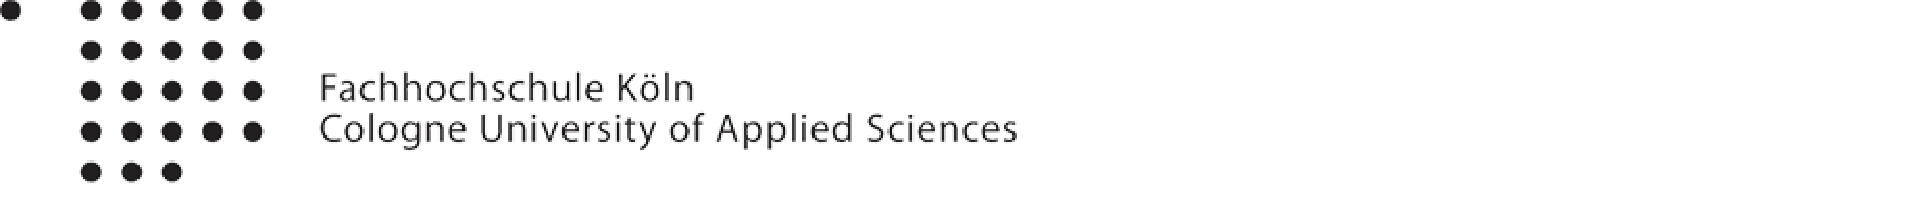
\includegraphics[natwidth=920pt, natheight=95pt, width=1.0\textwidth]{tex/logoheader.pdf}
\end{figure}

\vspace{2.0cm}

\begin{Huge}
	\textbf{WPF Compiler und Interpreter:}\\
	\vspace{0.1cm}
	\textbf{Java-Hardener}\\
\end{Huge}

\vspace{0.8cm}

\begin{LARGE}
	Abstrakt über einen Java-Postprozessor\\
	\vspace{0.1cm}
	zur automatisierten Bytecode-Manipulation\\
	\vspace{0.1cm}
	zur Reduzierung von \texttt{NullPointerException}s.\\
\end{LARGE}

\vspace{2.5cm}

\begin{tabular}{rl}
        Dozent:  &  Prof. Dr. Erich Ehses\\
       			 &  \small Fachhochschule Köln \\[1.0em]
\end{tabular}

\vspace{2.0cm}

\begin{large}
	ausgearbeitet von\\
	\vspace{0.2cm}
\end{large}

\begin{Large}
	Christoph Jerolimov, Matrikelnr. 11084742\\
	\vspace{0.5cm}
	Sommersemester 2013
\end{Large}

\end{center}

%Zeilenabstand für den Hauptteil ist 1,5 fach
\onehalfspacing

%=== Hauptteil =======================================================
%Seitennummerierung des Hauptteils
\mainmatter
	%Die Zähler für Tabellen und Abbildungen werden zurückgesetzt, damit
	%in jedem Kapitel die Nummerierung neu beginnt
	\setcounter{table}{1}
	\setcounter{figure}{1}
	%Einbinden des ersten Kapitels
	%!TEX root = ../Dokumentation.tex

\chapter{Abstrakt}

\texttt{NullPointerException}s (NPE) sind ein klassisches Problem der Softwareentwicklung
und treten in der Programmiersprache Java auf wenn Methoden- oder Attribut-Zugriffe
auf \texttt{null}-Object erfolgen\footnote{Dadrüber hinaus kann eine NPE auch
noch in anderen Fällen geworfen werden. Vgl. http://www.java-blog-buch.de/0503-nullpointerexception/}.

Die Behandlung solcher ungültiger Aufrufe ist grundsätzlich abhängig von der
Programmiersprache und der Laufzeitumgebung. So können entsprechende Zugriffe
zum Absturz des Programms führen, wie in Java zum werfen einer entsprechender
Ausnahme oder, wie etwa in Objective-C\footnote{Vgl. http://developer.apple.com/library/mac/documentation/Cocoa/Conceptual/ProgrammingWithObjectiveC/}, ignoriert werden.

Diese fehlertolerantere Version von Objective-C soll hier nachgebildet werden
und durch eine automatisierte manipulation des Java-Bytecodes erreicht werden.
Wie in der Vorlage müssen entsprechende Methoden immer einen Rückgabewert liefern,
hier werden, analog zu Objective-C, möglichst neutrale Werte gewählt:
False für boolsche Ausdrücke, Null für Zahlen und NULL-Referenzen für Objekte

Die beiden folgenden zwei Anwendungsfälle (vgl. Listing 1.1 und 1.2) verdeutlichen
die Einfachheit für den Programmier und würden ohne Bytecode-Manipulation
zu NullPointerExceptions führen.

\begin{lstlisting}[basicstyle=\ttfamily,numbers=left,numberstyle=\footnotesize\ttfamily,backgroundcolor=\color{source}]
List nullList = null;
System.out.println("List size: " + nullList.size());
\end{lstlisting}
\centerline{Listing 1.1: Beispiel für einen Null-Zugriff mit erwartetem Integer-Ergebnis}

\vspace{0.3cm}

\begin{lstlisting}[basicstyle=\ttfamily,numbers=left,numberstyle=\footnotesize\ttfamily,backgroundcolor=\color{source}]
List nullList = null;
if (!nullList.isEmpty()) {
	// Will run this code also if the nullList is null...
}
\end{lstlisting}
\centerline{Listing 1.2: Beispiel für einen Null-Zugriff mit erwartetem Boolean-Ergebnis}

\vspace{0.3cm}

Im folgendem werden verschiedene technische Möglichkeiten untersucht sowie
deren prototypische Umsetzung mithilfe der OpenSource Bibliothek ASM (siehe Kapitel 3) beschrieben.

Zur besseren Lesbarkeit wird auf Java-Packagenamen (etwa java.lang.) sowie Generics
in allen Java und Bytecode (Assembler) Darstellungen verzichtet. Alle angesprochenen
Dateien finden sich innerhalb dem diesem Projekt zugehörigem Sourcecode-Archiv.

 

\end{document}